\subsubsection{Neural Networks} \label{link::neural_networks}
Наиболее современным методом моделирования временных рядов как ранее описанных в настоящей работе, так и далее используемых в исследовании, является применение нейросетевого подхода, в основе которого лежит <<самообучающаяся>> функция, называемая нейронной сетью. 

Впервые предложенный Warren S. McCulloch и Walter Pitts \cite{mcculloch1943logical}, подход проведения вычислений сродни поведению нейрона стал набирать популярность как в областях применения: регрессия, классификация, кластеризация, так и в областях построения нейронных сетей. В 1961 году за счет трудов Frank Rosenblatt'а были изобретены многослойные персептроны \cite{rosenblatt1961principles}, за этим в 1980-х последовала разработка сверточных нейронных сетей, максимально эффективно --- на тот момент --- работающих с изображениями \cite{lecun1989backpropagation, lecun2015deep, lecun1989generalization}. После чего, когда речь зашла об обработке естественного языка были предложены рекуррентные нейронные сети, основанные не итеративном <<сборе информации>> о предоставляемых текстах \cite{hochreiter1997long, rumelhart1986learning}. 

В настоящий момент нейронные сети спокойно работают с видео, звуком, а также --- при определенных затратах вычислительных мощностей --- генерируют картинки. Однако State Of The Art (SOTA) почти во всех современных моделях глубокого обучения выступают трансформеры, в основе которых лежит механизм самовнимания \cite{attention_transformers}, позволяющий этим тяжелым сетям обрабатывать огромное количество информации, а что самое главное --- запоминать и вычленять ее. Однако в области прогнозирования временных рядом трансформеры пока что не занимают лидирующих позиций \cite{transformers_are_useless_for_TSF}.  Поэтому, так как в ценах/доходностях акций, конечно, содержится информация, которая позволяла бы применять подход контекстного анализа --- предсказываем то или иное слово в тесте, исходя из его контекста \cite{word2vec_2013}, однако она не носит лингвистический характер, что значительно усложняет сам процесс моделирования временного ряда. Именно по этой причине в настоящем исследовании не рассматривается применение трансформеров при построении прогноза временного ряда.

В настоящее время SOTA для работы с временными рядами является модель N~---~BEATS \cite{oreshkin2019n}, использующая в своей основе принцип нейронного бустинга \cite{schapire2003boosting}. Усовершенствованием данной модели является иной подход N~---~HiTS \cite{challu2022n}, основанный на вычленения долгосрочных паттернов из сигналов посредством реализации слоя MaxPooling с варьируемым размером ядра.

Замечаем, что в настоящем исследовании данные модели не рассматриваются, так как основная задача --- доказательство того, что нейросетевой подход дает более точный результат, чем эконометрический. Следовательно, выбор наиболее качественных и <<хороших>> моделей из области статистики и эконометрики предоставляем примерную точную верхнюю грань множества данных моделей, а выбор наиболее слабых нейровнных сетей --- примерную точную нижнюю грань множества нейронных сетей. Таким образом, подчеркиваем нецелесообразность включения в исследование моделей N~---~BEATS и N~---~HiTS, так как с большей вероятностью дают результат лучше. В противном случае, появляется качественное <<смещение>> результата.

\subsubsubsection{Multilayer Perceptron}
\\\\
\indent Ведя разговор о нейронных сетях, нельзя не затронуть сам способ построения подобных моделей. Впервые предложенный Frank Rosenblatt'ом \cite{rosenblatt1961principles}  в 1961 году принцип построения данных моделей, основанный на подобии того, как работает нейрон в мозгу человека, достаточно сильно изменялся, однако идея осталась прежней. По определению <<нейронная сеть>> --- последовательное преобразование признакового пространства. Соответственно формализованный вид данной операции имеет запись:
\begin{equation}
	a(X) = \phi_k(W_k \cdot \ldots \cdot \phi_2(W_2 \cdot \phi_1(W_1 X)))
\end{equation}
Где $W_j: j = \overline{1, k}$ --- некоторая матрица, в общем случае размер ее указать не удается, так как на каждом этапе вычисления получается переход в новое пространство с новой размерностью, $X \in \R^{n \times m}$ --- матрица объект-признак, используемая в качестве входных данных, а $\phi_j : j = \overline{1, k}$ --- используемая на конкретном слое функция активации. Сама же задача, появляющаяся перед исследователем имеет вид:
\begin{equation}
	\frac{1}{m} \sum_{j = 1}^m L(a(x_j | w), y_j) - R(w) \cdot \lambda \to \min_{w}
\end{equation}
Перед нами в общем случае невыпуклая огромная сумма, где $L(\cdot)$ --- функционал потерь, $w = \left\{W_1, \ldots, W_k\right\}$ --- не вектор, а просто набор данных, а $R(\cdot)$ --- функция регуляризации набора весов $w$, необходимая, чтобы уменьшить вероятность переобучения. Соответственно аналитически решение получить невозможно, однако существуют различного рода алгоритмы оптимизации, позволяющие достигать локального/глобального минимума итеративно. В общем случае интуиция, стоящая за достижением минимума, выглядит так:
\begin{equation}
	w^{t + 1} = w^t - \eta^t \cdot \nabla_w \left[L(a(x_j | w), y_j) - R(w) \cdot \lambda\right]
\end{equation}
Наиболее популярными в этой области являются Adam \cite{kingma2014adam}, AdamW \cite{bock2018improvement}, LBFGS \cite{liu1989limited}, а также недавно (2023 год) разработанный Lions \cite{chen2023symbolic}. В настоящем исследовании применяются исключительно LBFGS (для обучения MLP), а также --- в случаях, когда LBFGS дает неудовлетворительный результат --- AdamW как наиболее распространенный (универсальный) его заменитель.

Сама идея алгоритма обучения завязана на применение теоремы о дифференцировании сложной функции, так как $a(\cdot)$ именно ей и является. Таким образом, для вычисления такого количества производных используется алгоритм под названием BackPropagation \cite{linnainmaa1970representation}. Принцип его работы заключается в дифференцировании графа вычислений, схематично представляющего исходную нейронную сеть. В формальном виде:
\begin{equation}
	\frac{\partial L}{\partial w} = \left. \frac{\partial f_1}{\partial w} \right\rvert_w \left. \frac{\partial f_2}{\partial f_1} \right\rvert_{f_1(w)} \cdot \ldots \cdot \left. \frac{\partial f_k}{\partial f_{k - 1}} \right\rvert_{f_{k - 1}(\cdot)} \left. \frac{\partial L}{\partial f_k} \right\rvert_{f_k\left(f_{k - 1}(\cdot)\right)} = \nabla_w L
\end{equation}
Интересно отметить, что существует теорема, гласящая, что, имея однослойную нейронную сеть, можно с любой точностью приблизить абсолютно любую непрерывную функцию многих переменных \cite{cybenko1989approximation}.

В качестве примера рассматриваем способность к прогнозированию на один рабочий день биржи модели MLP для цен акций открытия компании Ford, начиная с даты выхода компании на IPO, а заканчивая 13/12/2022 годом.
\begin{figure}[H]
	\centering
	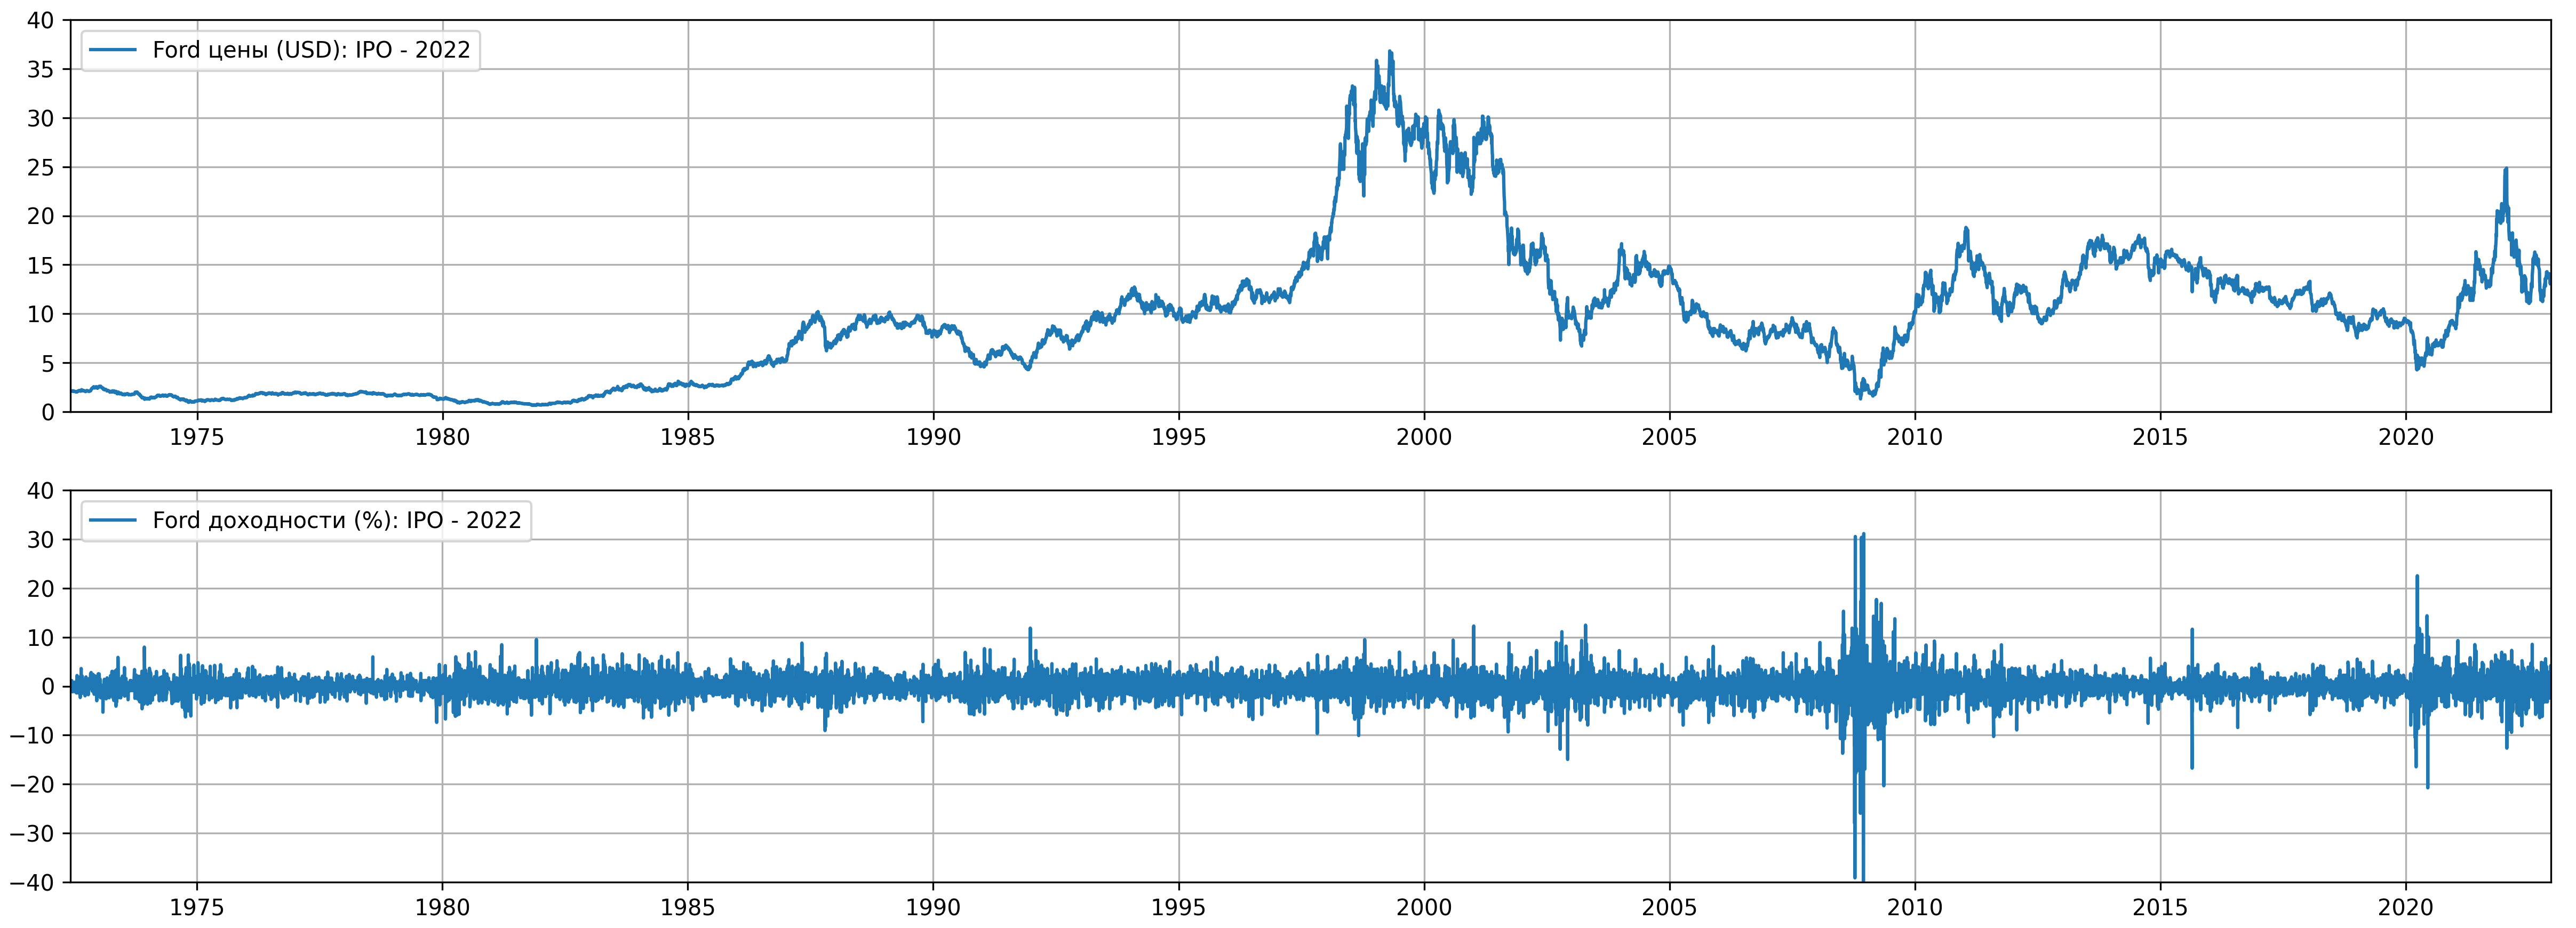
\includegraphics[width=17cm]{returns pictures/ford_prices_returns.png}
	\caption{График цены открытия и доходности Ford (IPO --- 2022)}
	\label{fig::ford_prices_returns}
\end{figure}
Далее смотрим на показатели функции потерь для обучающей выборки и валидационной по мере обучения самой модели. В качестве функции потерь в данном случае используется уже ранее обсуждавшаяся MSE, а в качестве метрики выбрана WAPE (Weighted Average Percentage Error):
\begin{figure}[H]
	\centering
	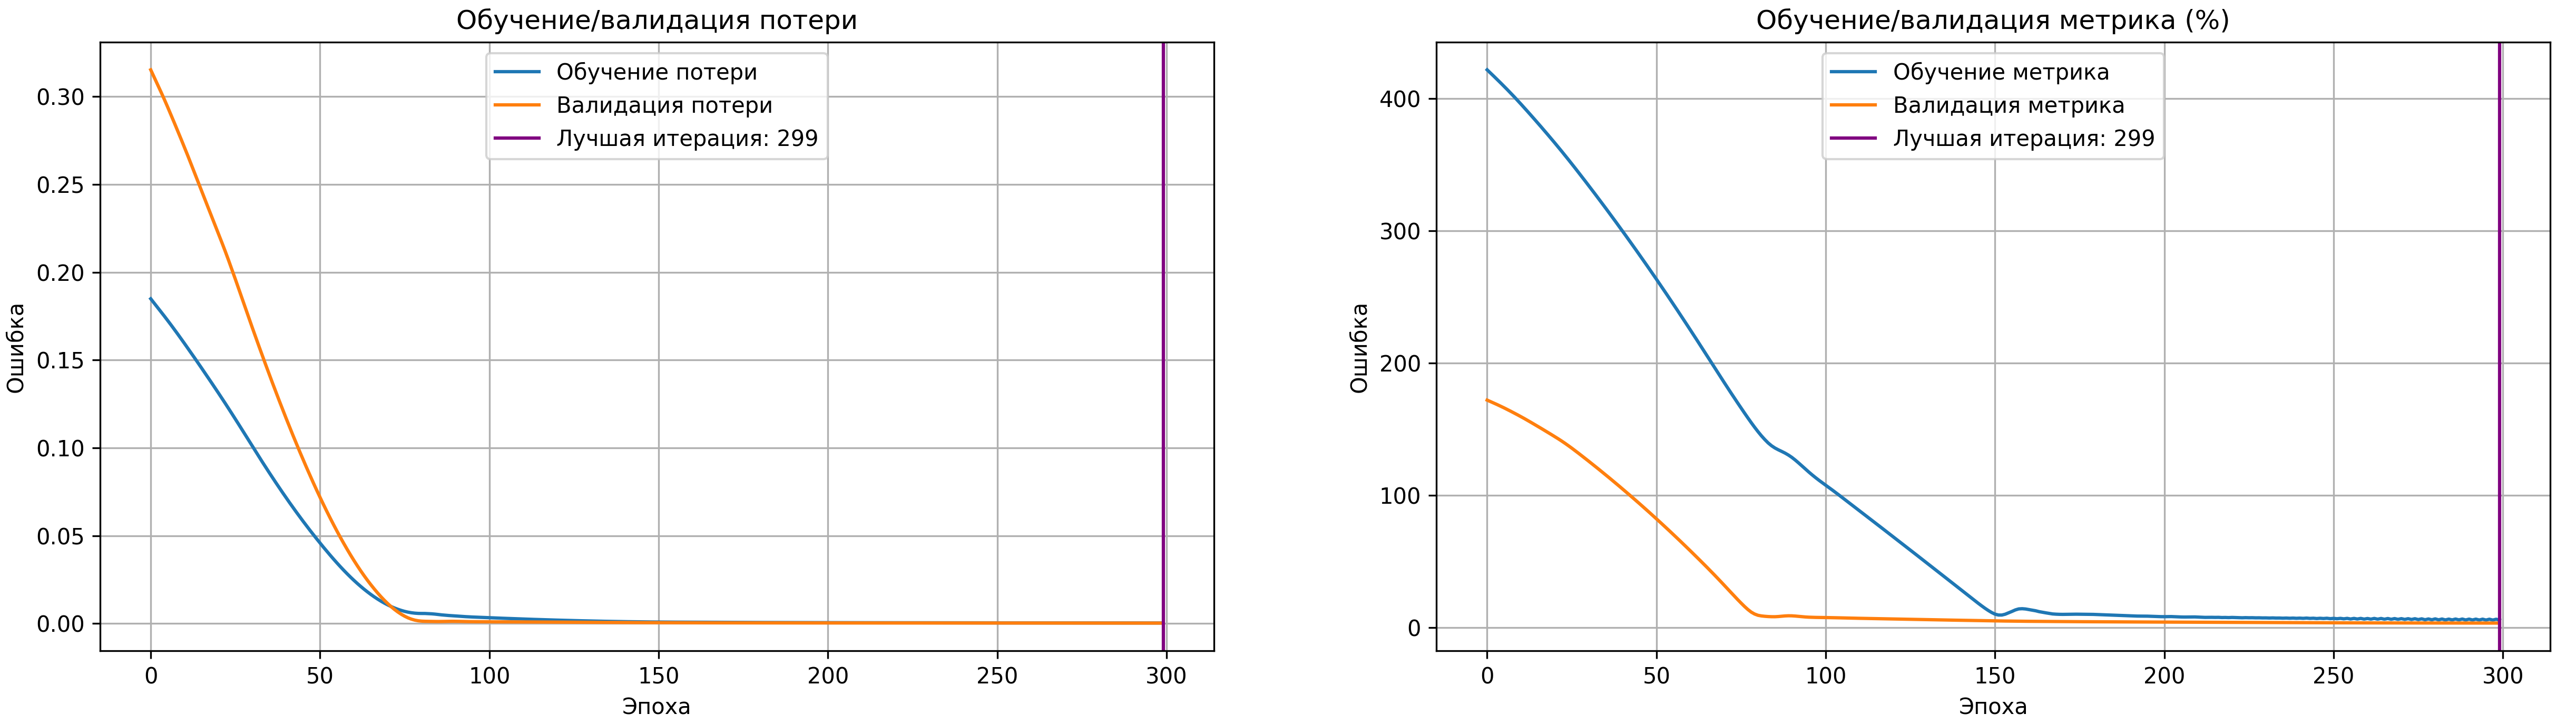
\includegraphics[width=17cm]{nn/mlp/ford_train_val_results.png}
	\caption{График MSE для модели MLP}
	\label{fig::ford_train_val_results}
\end{figure}
Но также интересно, как менялось значение лучшей валидационной метрики, ведь именно она является критерием сохранения весов модели. Принцип прост: если меньше максимального, сохраняй модель. Более подробно: после прохода по всей обучающей выборке (то есть после прохождения <<эпохи>>) происходит валидационный цикл, во время которого вычисляется WAPE. Если WAPE на шаге $t$ меньше, чем WAPE на шаге $t - 1$, то веса, полученные в модели на момент $t$ сохраняются в отдельный файл. После чего перед началом тестового цикла, во время которого вычисляется WAPE для тестовых данных, происходит <<загрузка>> в модель полученных на <<лучшей>> итерации весов, исходя из которых далее получается финальное значение выбранной метрики --- в нашем случае, WAPE.
\begin{figure}[H]
	\centering
	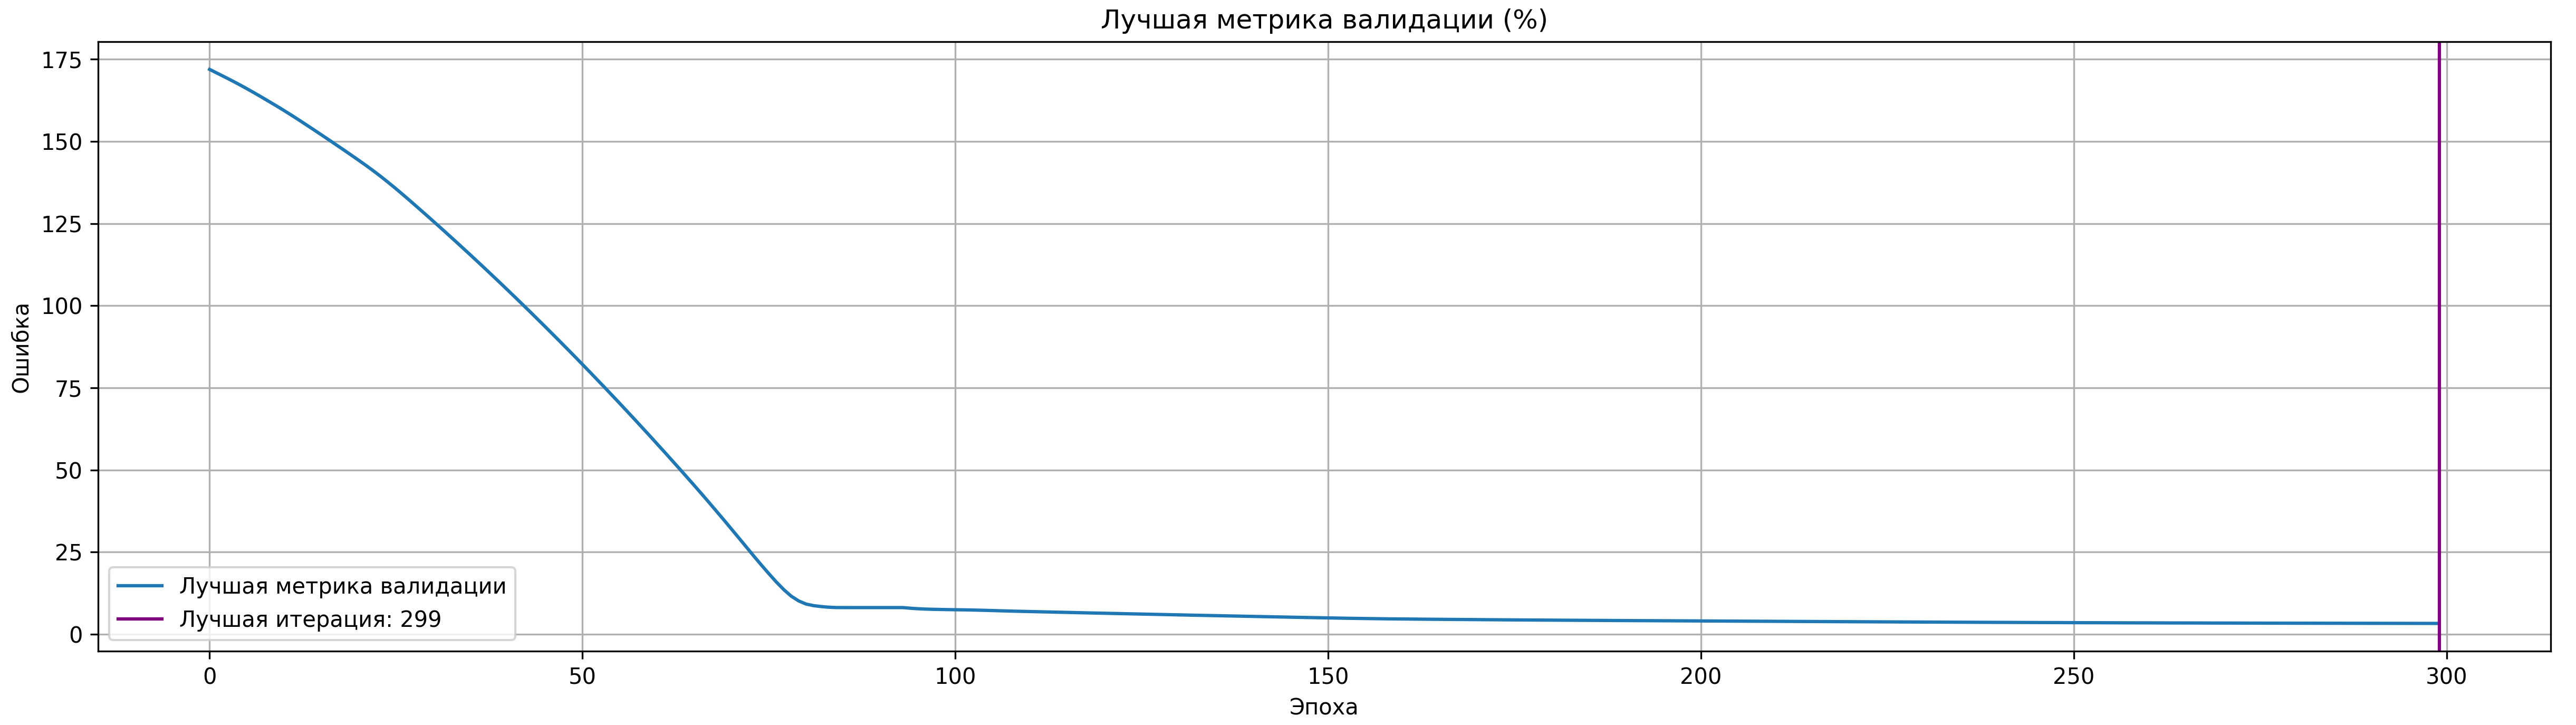
\includegraphics[width=17cm]{nn/mlp/ford_best_metric_results.png}
	\caption{График изменения лучшей валидационной метрики: WAPE$(y, \hat{y}) = \sum_{t = 1}^n |y_t - \hat{y}_t| / \sum_{t = 1}^n |y_t|$}
	\label{fig::ford_train_best_metric_results}
\end{figure}
Финальным этапом является построение прогноза и подсчета получившейся ошибки в терминах процентного отклонения WAPE и аналогично ранее указанной RMSE.
\begin{figure}[H]
	\centering
	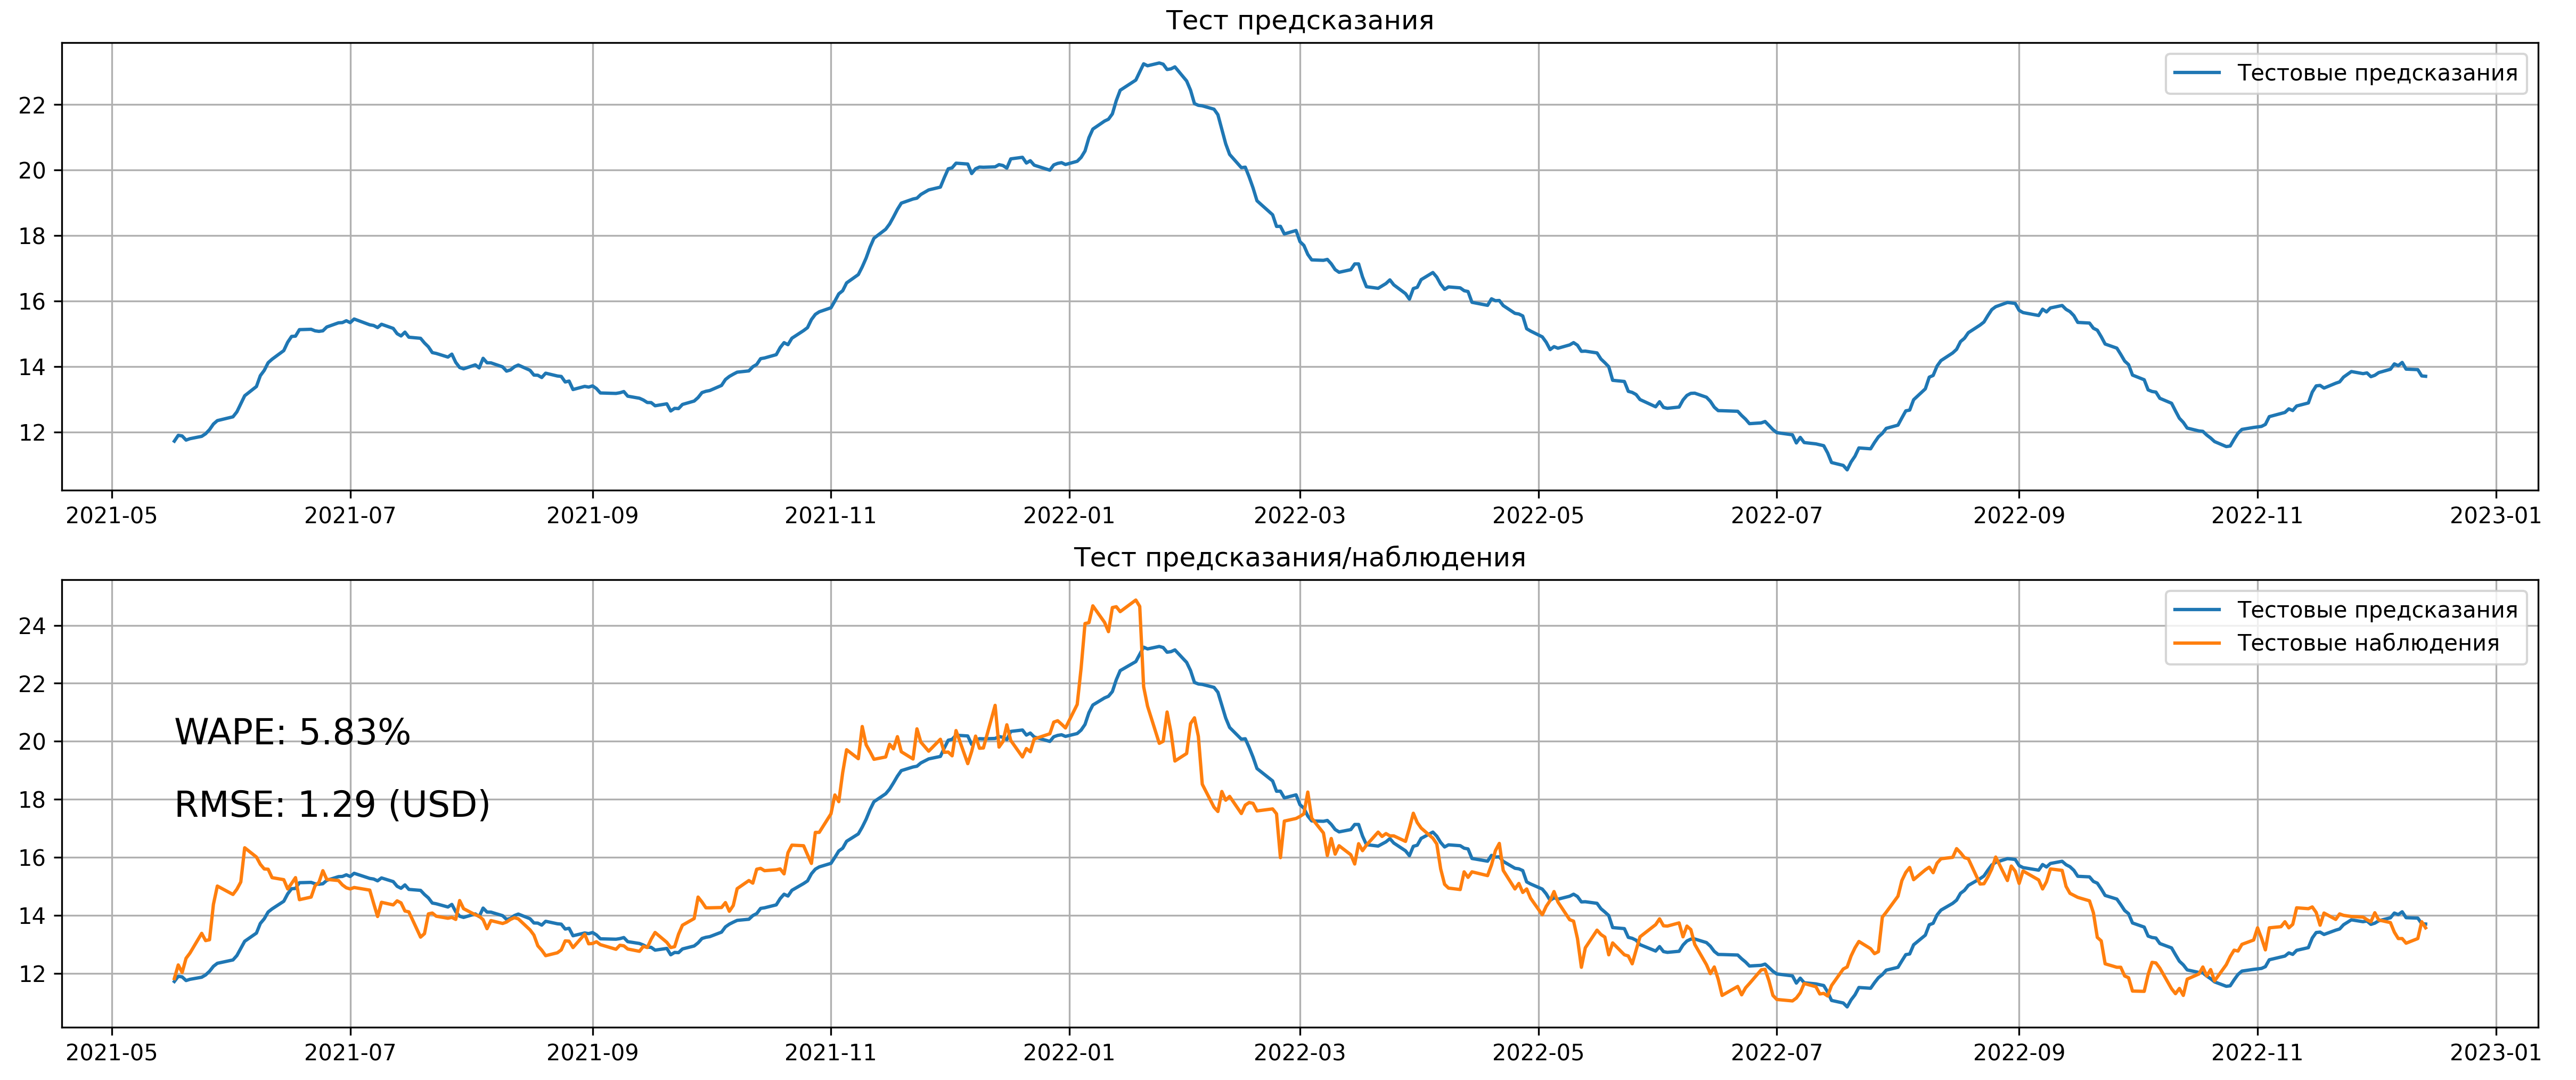
\includegraphics[width=17cm]{nn/mlp/ford_test_results.png}
	\caption{График реальных и предсказанных значений цен акций Ford (USD)}
	\label{fig::ford_test_results}
\end{figure}
Очевидно, что методика неплохо работает, так как полученная метрика без наличия тюнинга (подбора гиперпараметров) составляет $\pm 1.29$ USD, что достаточно мало, но существенно в случае большого количества акций, с которыми совершается операция. Нельзя сказать, что полученный результат является неприменимым к жизненным ситуациям, хотя без оговорок не обойтись: ошибка слишком велика в денежном эквиваленте, таким образом, лучше опираться на выводы полученной модели при оперировании небольшой суммой денег, так как сама по себе ошибка растет прямо пропорционально сумме операции. Однако остается провести аналогичное исследование для доходностей, чтобы в полной мере понять способность модели к прогнозированию. Так как обучение модели на ценах, исходя из визуального анализа графика, кажется более естественным по причине наличия некоторого тренда, нежели аналогичное действие по отношению к доходностям в условиях их волатильности и резких изменений. Другими словами, доходности более похожи на звуковую дорожку, чем на некоторый процесс.
\begin{figure}[H]
	\centering
	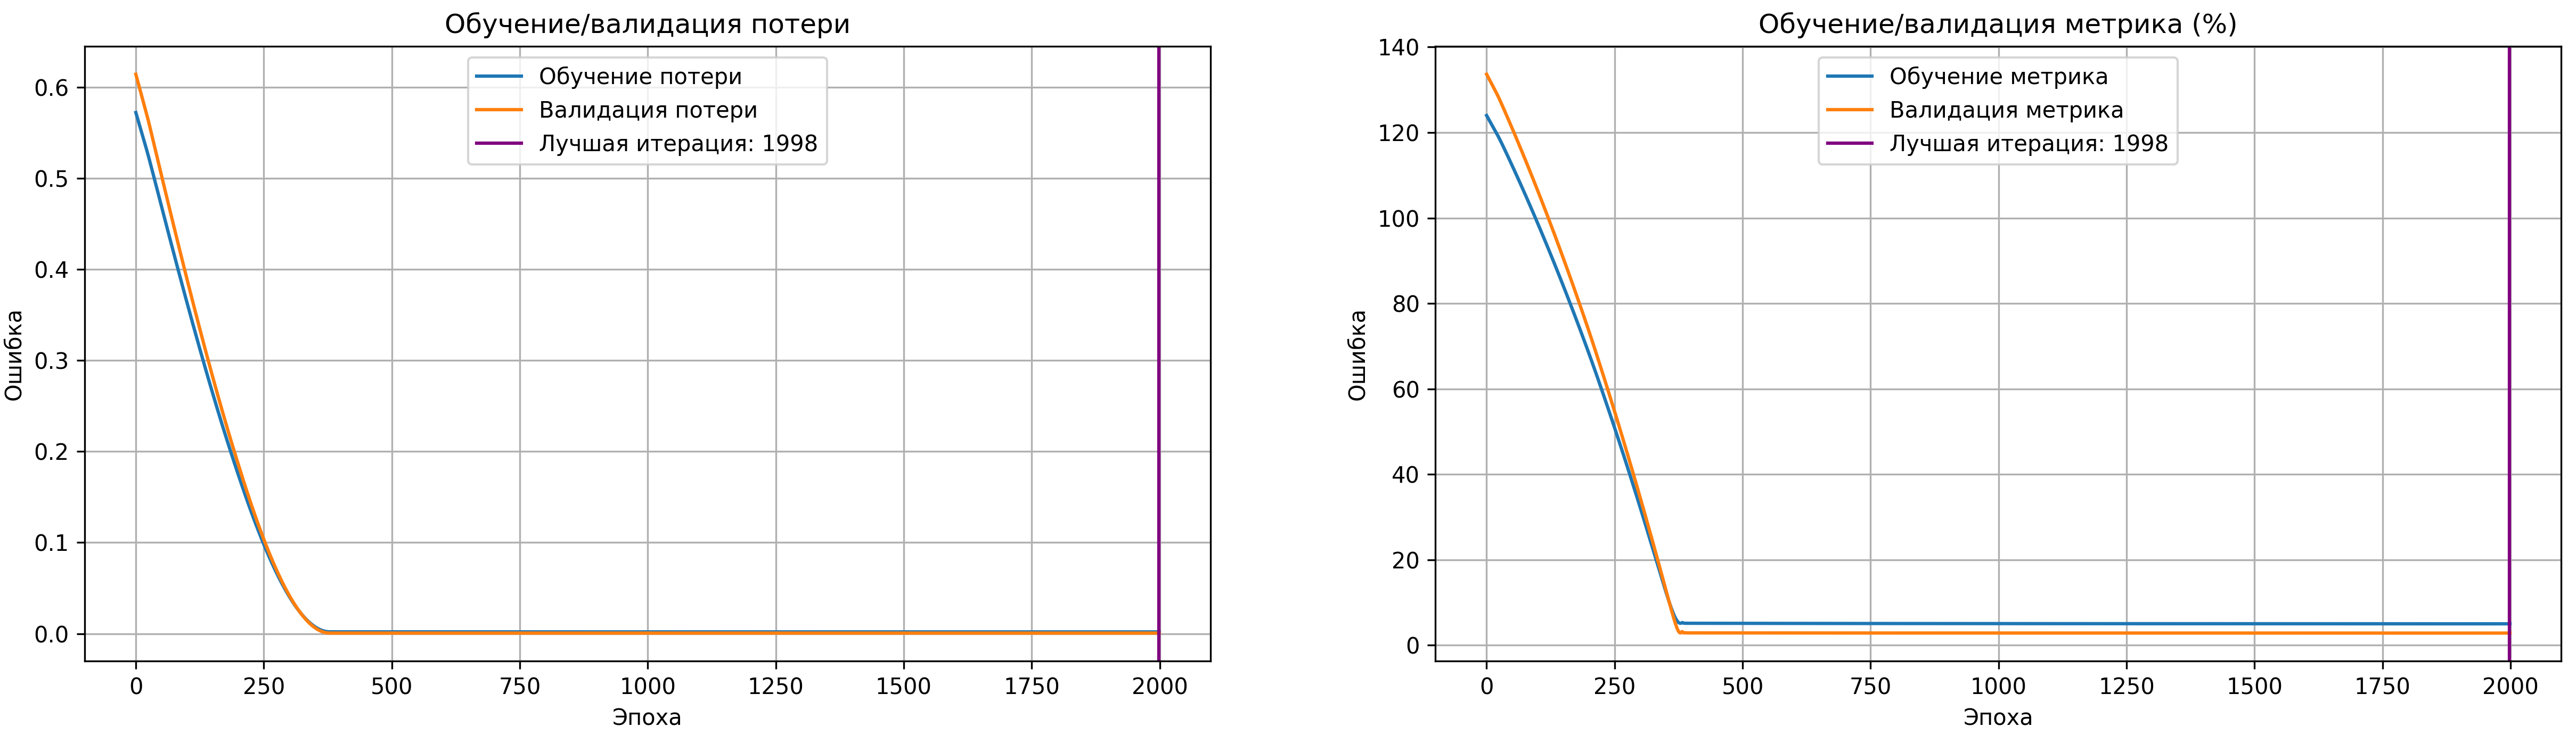
\includegraphics[width=17cm]{nn/mlp/ford_train_val_returns_results.png}
	\caption{График MSE для модели MLP (доходности \%)}
	\label{fig::ford_train_val_returns_results}
\end{figure}
Поведение достаточно схожее с моделью на ценах, то есть обучение выполняется достаточно успешно. Однако пока что это ничего не говорит о самом поведении модели на тестовой выборке, ведь данная кривая символизирует лишь успешную сходимость к минимуму. То есть даже, если ошибка мала, результат может быть неудовлетворительным, из-за необходимости обоснования поведения обученной модели, исходя из логической составляющей, прикладываемой к реальности. Иными словами, полученные результаты должны согласовываться с реальностью, даже если показатель ошибки минимален.
\begin{figure}[H]
	\centering
	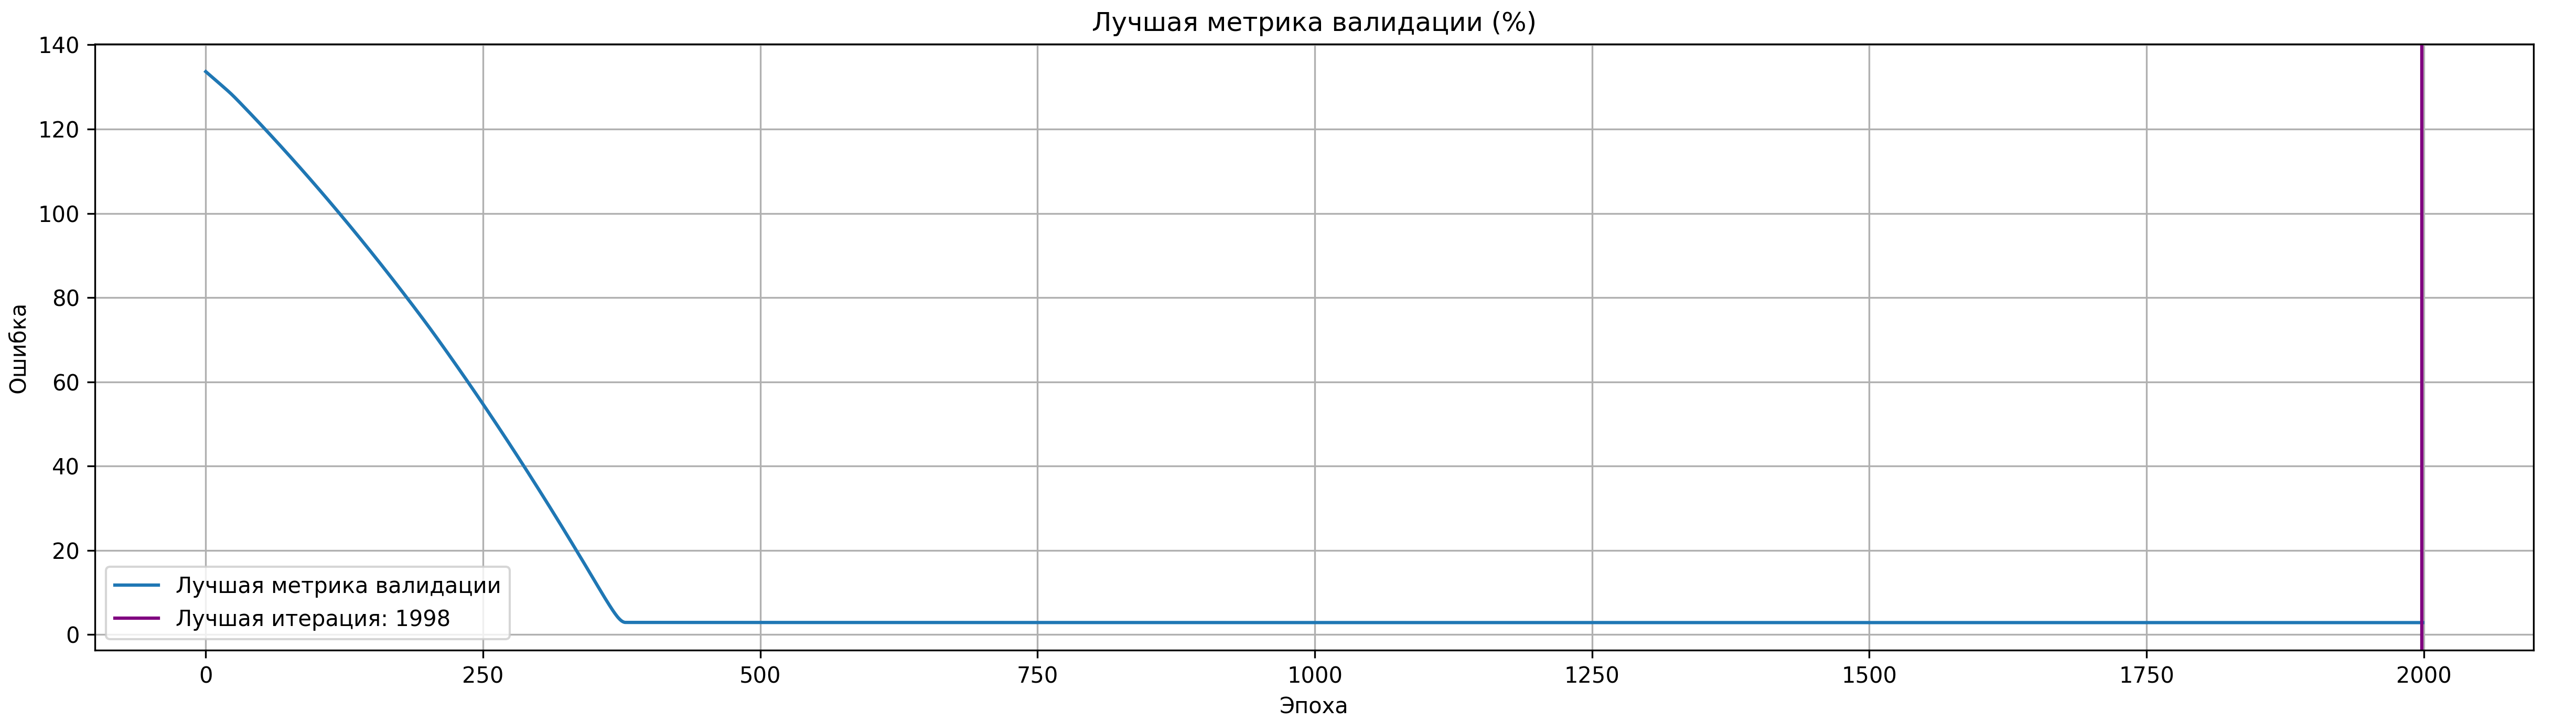
\includegraphics[width=17cm]{nn/mlp/ford_best_metric_returns_results.png}
	\caption{График изменения лучшей валидационной метрики: WAPE$(y, \hat{y}) = \sum_{t = 1}^n |y_t - \hat{y}_t| / \sum_{t = 1}^n |y_t|$ (доходности \%)}
	\label{fig::ford_best_metric_returns_results}
\end{figure}
Видим, что ошибка по мере продвижения по эпохам ведет себя <<хорошо>>, то есть достаточно стремительно убывает, однако на 375 итерации выходит на плато. Соответственно, изменение ошибки на данном плато достаточно мало, следовательно, необходимо либо динамически изменять скорость обучения (выше описанный параметр $\lambda$, он же learning rate --- далее lr) или изначально брать lr больше, чтобы <<проскочить>> достигнутый минимум. Дополнительный вариант действий, который может привести к улучшению результата --- использование либо более сложной архитектуры, либо более простой, чтобы видоизменить поверхность функции потерь, по которой <<скатывается>> ее градиент. Теперь, опираясь на сказанное ранее, смотрим на предсказания для тестовой выборки, из которых далее делаем вывод о качестве работы обученной модели.
\begin{figure}[H]
	\centering
	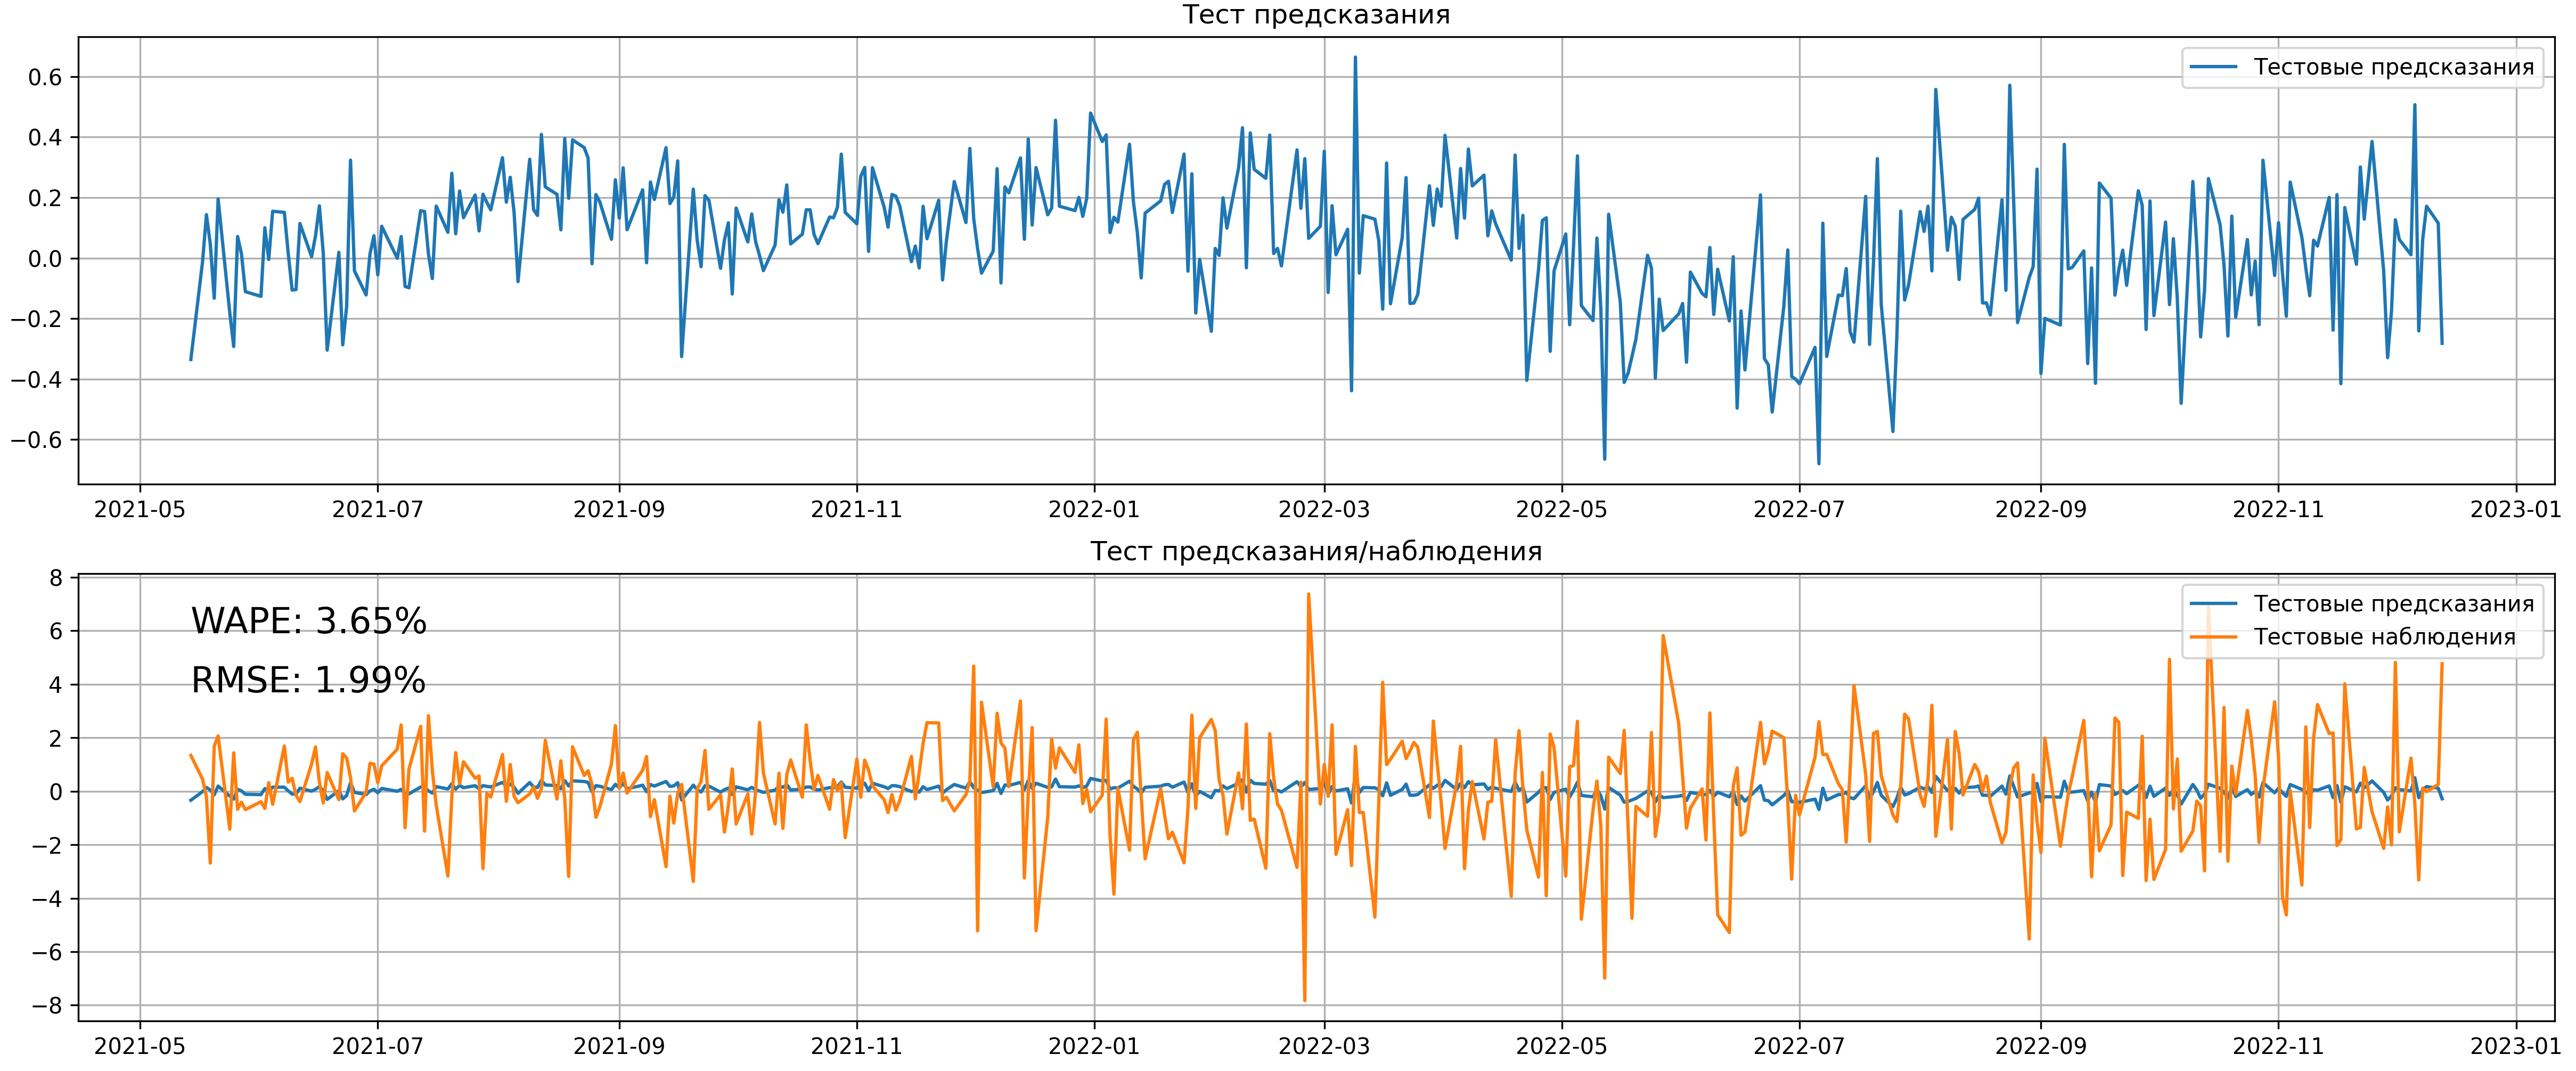
\includegraphics[width=17cm]{nn/mlp/ford_test_returns_results.png}
	\caption{График реальных и предсказанных доходностей акций Ford (\%)}
	\label{fig::ford_test_returns_results}
\end{figure}
Очевидно, что полученный результат, хотя и полученная ошибка мала, не является удовлетворительным и применимым к реальности, так как, основываясь на метрике RMSE, имеем отклонение $\pm 1.99\%$, что заметно больше, чем средняя предсказанная величина. Таким образом, настоящая модель не только не может быть применена к реальности, но и способна ввести в заблуждение относительно ответа на вопрос <<Buy, Hold or Sell>>.

Также замечаем, что поведение предсказанных показателей как будто сдвинуто немного вперед. То есть в реальности уже было, а в прогнозе --- только будет. Подобное возможно по трем причинам: малая мощность модели, непригодность модели, особенность рассматриваемых данных. Значит, нельзя делать поспешные выводы о качестве самой модели, ведь анализ велся только для одной компании. Финальный ответ о пригодности той или иной модели рассматривается в заключении настоящего исследования. Однако текущая модель включается в финальную таблицу как способная к прогнозированию как цен, так и доходностей.
\subsubsubsection{Recurrent Neural Network}
\\\\
\indent Развивая тему особенностей архитектур сетей, задаемся вопросом: \textbf{Q}: MLP работает с матрицей вида объект---признак, однако как поступать в случае работы с временным рядом, ведь исходный его вид --- просто вектор? \textbf{A}: Как уже отмечалось в блоке Singular Spectrum Analysis (\myref{link::ssa}), переводим имеющийся ряд (вектор) в матричное пространство посредством применения алгоритма подобного ханкелизации. Таким образом, вместо временного ряда $y \in \R^{N}$, получаем матрицу $y \in \R^{L \times K}$, где $K  = N - L$. Для большей наглядности рассматриваем пример.
\begin{equation}
	\begin{split}
		y = \left[\begin{matrix}
			1\\2\\3\\4\\5\\6
		\end{matrix}\right], L = 4, K = 6 - 4 = 2 \Rightarrow
		X = \left[\begin{matrix}
			1 & 2\\
			2 & 3\\
			3 & 4\\
			4 & 5\\
		\end{matrix}\right]
		y = \left[\begin{matrix}
			3\\
			4\\
			5\\
			6\\
		\end{matrix}\right]
	\end{split}	
\end{equation}
Получаем то, что было нужно. Матрица объект-признак ($X$) и вектор выходов ($y$), который должен быть в итоге. Однако снова появляется вопрос \textbf{Q}: Так как работа ведется с временным рядом, целесообразно ли иметь фиксированный набор признаков, который подается на вход сети. В текущих условиях входной размерностью сети является величина $K$ (количество временных лагов). Но, что будет, если два лага найдутся не всегда? \textbf{A}: Решением этой проблемы является способ построения нейронных сетей, предложенный в \cite{hochreiter1997long, rumelhart1986learning}, представляющий из себя пошаговый сбор информации о последовательности. Данный поход получил название Recurrent Neural Network (рекуррентная нейронная сеть).

Идея в том, что на вход аналогично всему предыдущему подается наблюдение, однако, рассуждая абстрактно, имеется в виду не просто \textit{одно} наблюдение, а последовательность из них. Для лучшего понимания происходящего рассматриваем пример выше. Чтобы перевести имеющиеся $X$ и $y$ в требуемые для RNN размерности, выполняем операцию:
\begin{equation}
	\begin{split}
		X = \left[\begin{matrix}
			1 & 2\\
			2 & 3\\
			3 & 4\\
			4 & 5\\
		\end{matrix}\right]
		y = \left[\begin{matrix}
			3\\
			4\\
			5\\
			6\\
		\end{matrix}\right]
		\Rightarrow
		X = \left[\begin{matrix}
			[1], & [2]\\
			[2], & [3]\\
			[3], & [4]\\
			[4], & [5]\\
		\end{matrix}\right]
		y = \left[\begin{matrix}
			[3]\\
			[4]\\
			[5]\\
			[6]\\
		\end{matrix}\right]
	\end{split}	
\end{equation}
То есть теперь $X \in \R^{L \times K \times 1}$, а значит, приводя все в соответствие необходимой терминологии, $L$ --- размер батча, $K$ --- длина последовательности, $1$ --- количество имеющихся признаков у одного наблюдения, в нашем случае --- цена акции открытия, однако возможно наличие и других составляющих. А теперь самое интересное: подобная архитектура требует лишь фиксированного количества признаков у одного наблюдения, в то время как длина последовательности --- количество лагов, в нашем случае --- остается динамической. Следовательно, не нужно менять архитектуру сети в зависимости от количества используемых лагов --- в зависимости от длины последовательности. Данные подготовлены, теперь приступаем к систематическому изложению особенности работы алгоритма RNN.

Существует на данный момент три основных блока рекуррентных сетей: Simple Recurrent Unit \cite{rumelhart1986learning}, Long Short Term Memory (LSTM) \cite{hochreiter1997long}, Gated Recurrent Unit (GRU) \cite{cho2014learning}. Коротко говоря о каждом из них, привожу иллюстративный способ работы блоков, а также формальные вычисления.

Для начала --- Simple Recurrent Unit:
\begin{figure}[H]
	\centering
	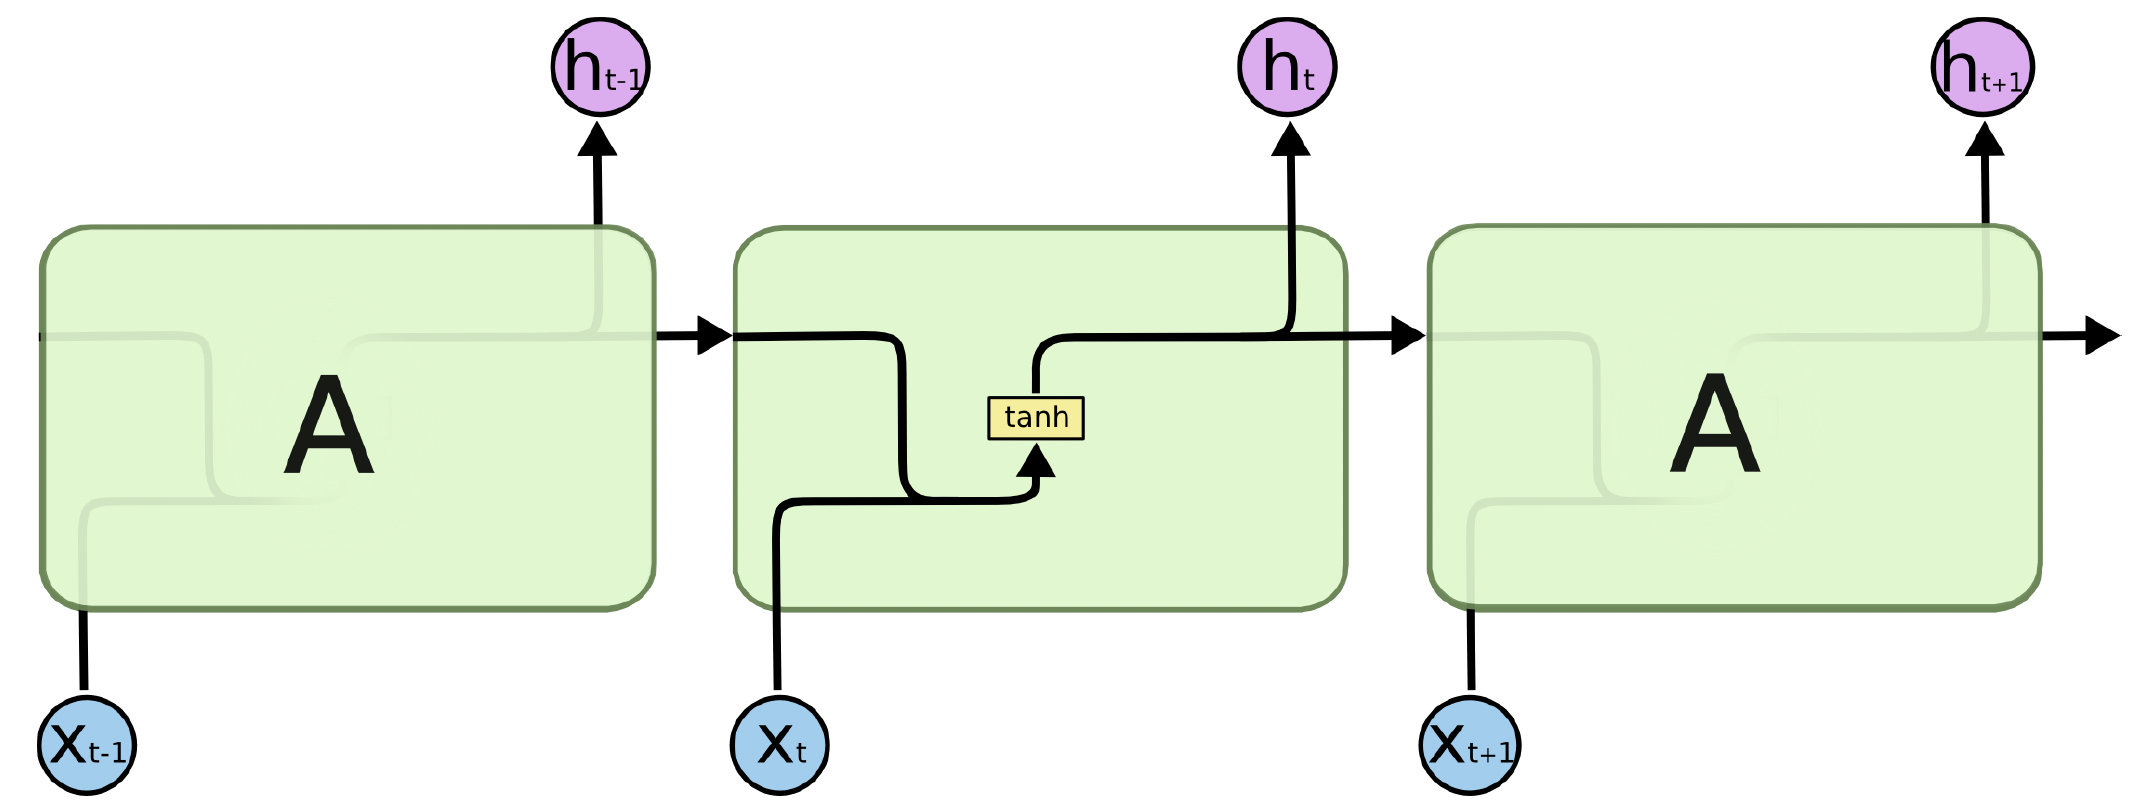
\includegraphics[width=17cm]{nn/rnn/units/rnn_unit.png}
	\caption{Визуализация блока Simple Recurrent Unit}
	\label{fig::rnn_unit}
\end{figure}
\noindent В формальном виде, вычисления проходят следующим образом:
\begin{equation}
	\begin{split}
		h_t & = \sigma\left(W_{hh}h_{t - 1} + W_{hx} x_t + b_h\right)\\
		y_ t & = g\left(W_{yh}h_t + b_y\right)
	\end{split}
\end{equation}
Но тут сразу встает вопрос о затухании градиента при обратном проходе, то есть при применении так называемого алгоритма BackPropagation Through Time (BPTT), являющегося аналогичным классическому BackPropagation \cite{linnainmaa1970representation}. Формально данный вывод получаем посредством дифференцирования выбранной функции потерь:
\begin{equation}
	\begin{split}
		\frac{\partial L}{\partial w} = \sum_{t = 1}^T  \frac{\partial h_k}{\partial w} \left\{ \prod_{i = k + 1}^{t} \frac{\partial h_i}{\partial h_{i - 1}}\right\} \frac{\partial y_t}{\partial h_t} \frac{\partial L}{\partial y_t}
	\end{split}
\end{equation}
При этом если $\lVert \frac{\partial h_i}{\partial h_{i - 1}} \rVert_2 > 1 \Rightarrow$ взрыв, иначе $\lVert \frac{\partial h_i}{\partial h_{i - 1}} \rVert_2 < 1 \Rightarrow$ затухание в силу наличия произведения матриц Якоби. При этом --- желаемый результат --- $\lVert \frac{\partial h_i}{\partial h_{i - 1}} \rVert_2 = 1$. Решением появившейся проблемы стало изобретение в 1991 блока Long Short Term Memory, описанного в \cite{hochreiter1991untersuchungen, hochreiter1997long}. В формальном виде процесса вычислений получаем:
\begin{equation}
	\begin{split}
		f_t & = \sigma \left(W_{hh}^f h_{t - 1} + W_{hx}^f x_t + b_h^f\right)\\
		i_t & = \sigma \left(W_{hh}^i h_{t - 1} + W_{hx}^i x_t + b_h^i\right)\\
		o_t & = \sigma \left(W_{hh}^o h_{t - 1} + W_{hx}^o x_t + b_h^o\right)\\
		\tilde{c}_t & = \tanh\left(W_{hh}^c h_{t - 1} + W_{hx}^c x_t + b_c\right)\\
		c_t & = f_t c_{t - 1} + i_{t} \tilde{c}_t\\
		h_t & = o_t \tanh\left(c_t\right)
	\end{split}
\end{equation}
\noindent Графически же иллюстрация вычислительного процесс имеет более сложный вид, чем выше упомянутый Simple Recurrent Unit, однако сложность архитектуры окупается способностью данного блока избегать проблемы затухания градиента, а также --- способностью вычленять долгосрочные зависимости в имеющихся данных (в терминах сигналов --- выделение тренда).
\begin{figure}[H]
	\centering
	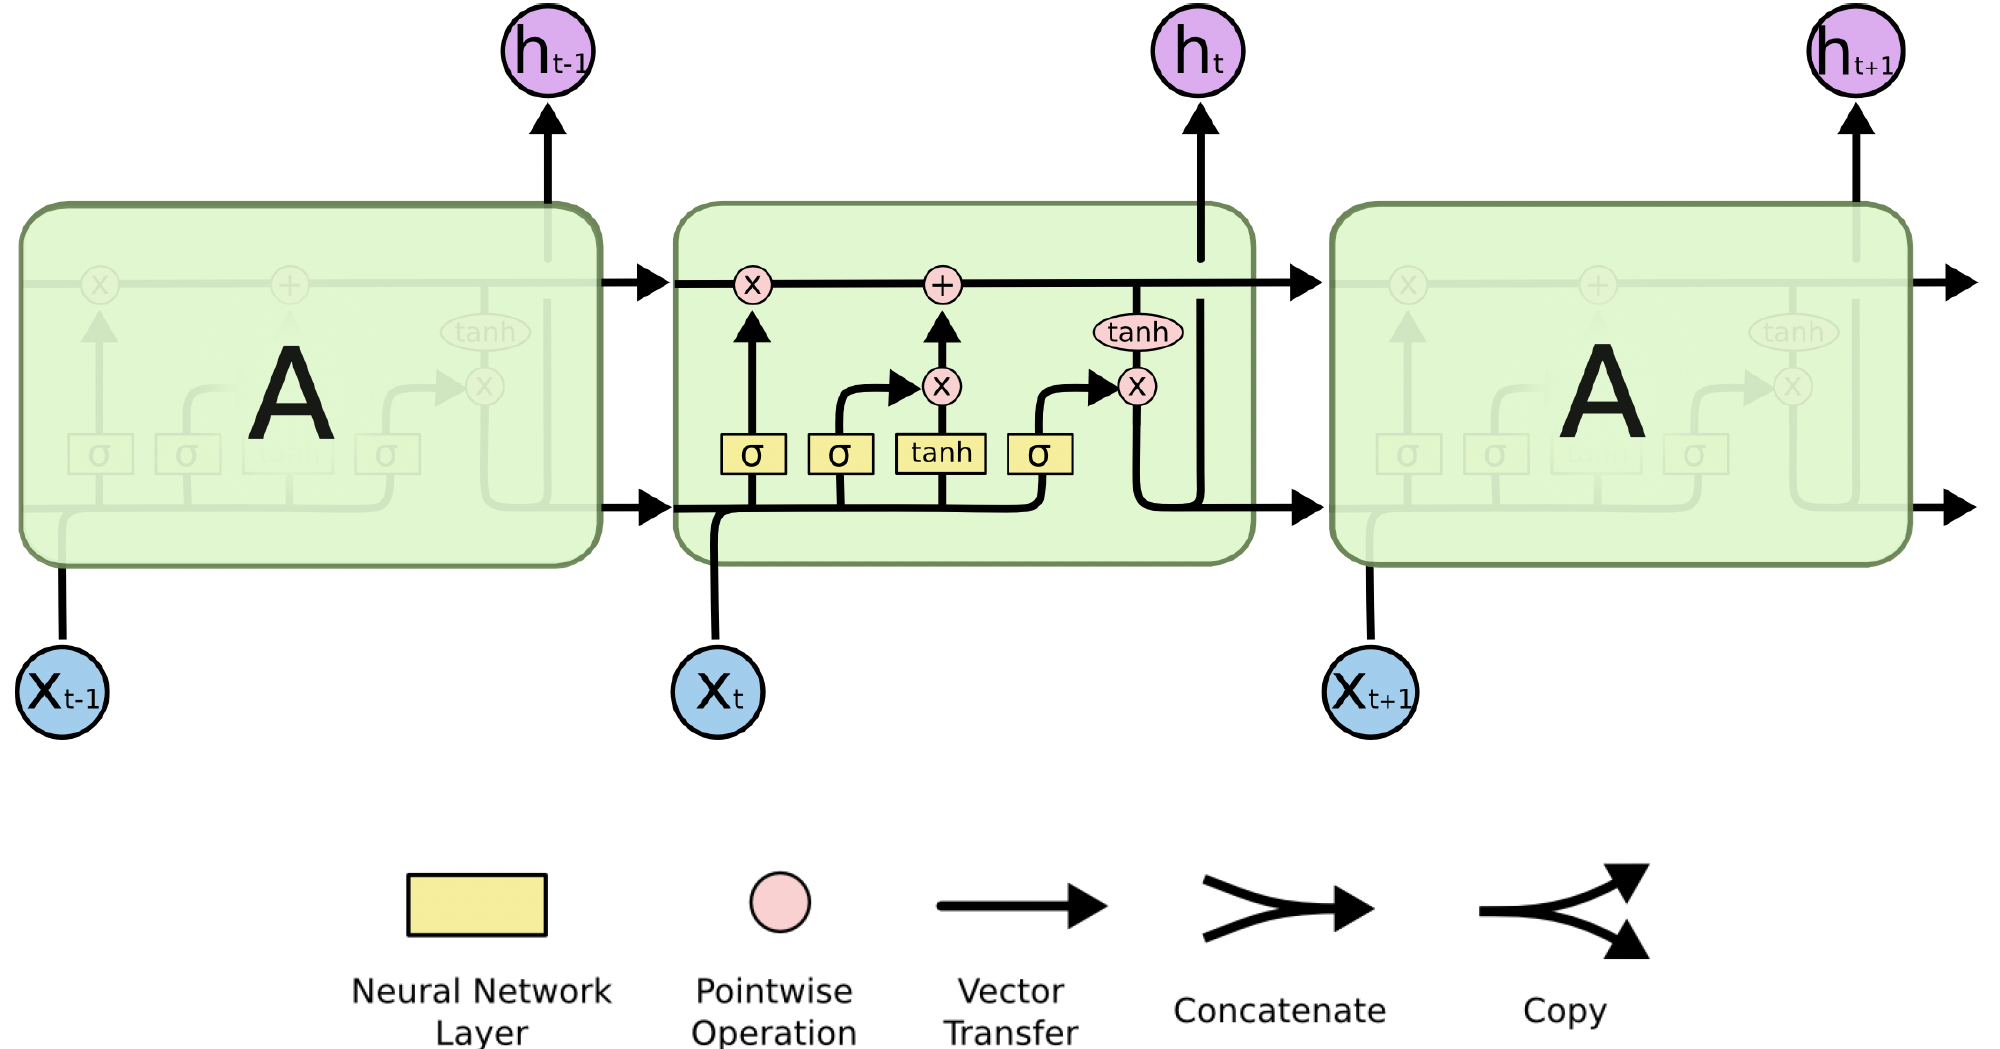
\includegraphics[width=17cm]{nn/rnn/units/lstm_unit.png}
	\caption{Визуализация блока Long Short Term Memory}
	\label{fig::lstm_unit}
\end{figure}
Как видим, проблема с затуханием градиента решена, однако блок получился достаточно тяжелым с точки зрения вычислений и, более того, проблема <<взрыва>> градиента никуда не делать. Вторая трудность решается посредством приема, называемого gradient clipping \cite{mikolov2012statistical}, а первая, в свою очередь, посредством далее изобретенного в 2014 блока Gated Recurrent Unit \cite{cho2014learning}, который по качеству работы сравним с LSTM, но при этом является более <<легким>> в плане количества обучаемых параметров. Формулы данного процесса:
\begin{equation}
	\begin{split}
		z_t & = \sigma\left(W_{hh}^i h_{t - 1} + W_{hx}^i x_t + b_h^z\right)\\
		r_t & = \sigma\left(W_{hh}^r h_{t - 1} + W_{hx}^r x_t + b_h^r\right)\\
		\tilde{h}_t & = \tanh \left(W_{hh}^r h_{t - 1} + W_{hx}^r x_t\right)\\
		h_t & = (1 - z_t) h_{t - 1} + z_t \tilde{h}_t
	\end{split}
\end{equation}
\noindent Визуально реализация блока GRU выглядит намного легче в плане количества параметров, чем LSTM, что позволяет предполагать увеличение скорости обучения сети, но при этом сохранение качества получаемых результатов.
\begin{figure}[H]
	\centering
	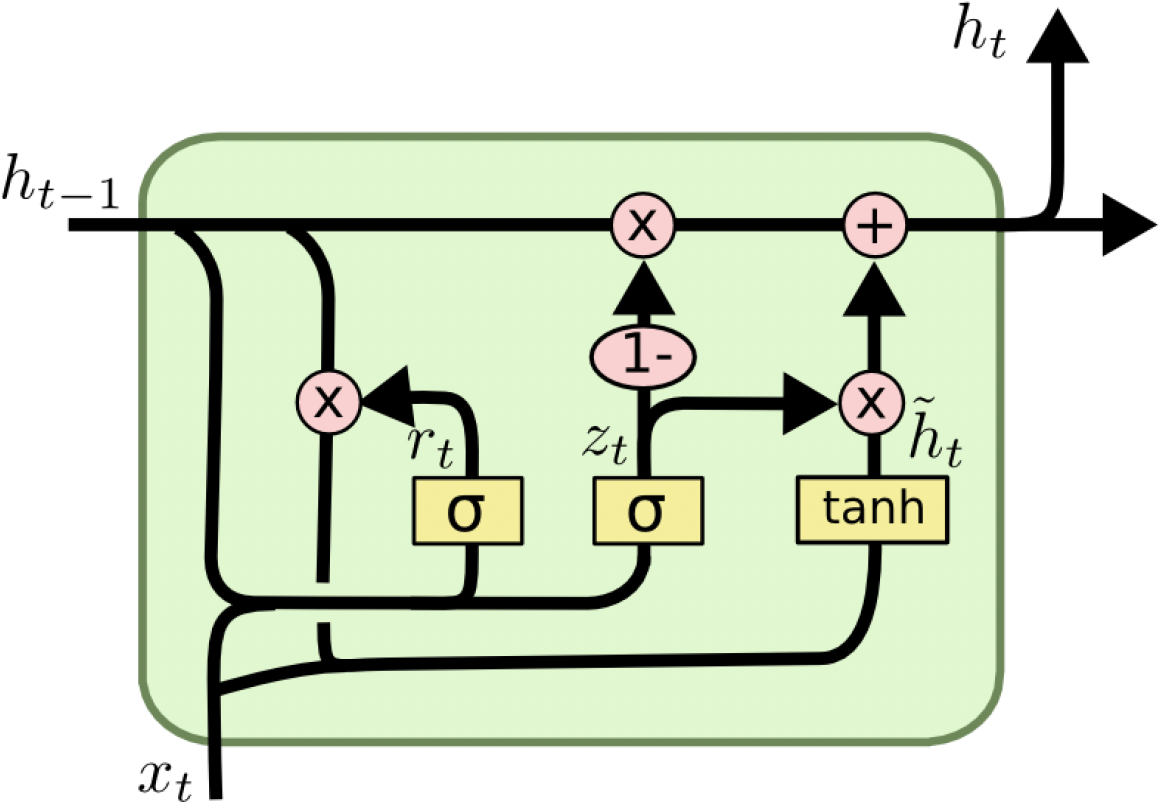
\includegraphics[width= 8cm]{nn/rnn/units/gru_unit.png}
	\caption{Визуализация блока Gated Recurrent Unit}
	\label{fig::gru_unit}
\end{figure}
Несмотря на все достоинства GRU перед LSTM невозможно однозначно сказать, какой из указанных блоков лучше. Таким образом, остается лишь один способ проверки --- эмпирически на имеющихся данных. В настоящей работе в качестве примера приводится эмпирический анализ каждого из выше указанных блоков на имеющихся данных о ценах открытия компании Ford.

Ниже приводим полученные результаты для блока Simple Recurrent Unit.
\begin{figure}[H]
	\centering
	\includegraphics[width= 17cm]{nn/rnn/block_results/rnn/ford_train_val_prices.png}
	\caption{График MSE для блока Simple Recurrent Unit (цены USD)}
	\label{fig::rnn_ford_train_val_prices}
\end{figure}
\noindent Далее смотрим на динамику лучшей валидационной метрики за все время обучения:
\begin{figure}[H]
	\centering
	\includegraphics[width= 17cm]{nn/rnn/block_results/rnn/ford_best_metric_prices.png}
	\caption{График изменения лучшей валидационной метрики: WAPE}
	\label{fig::rnn_ford_best_metric_prices}
\end{figure}
\noindent Далее --- предсказания:
\begin{figure}[H]
	\centering
	\includegraphics[width= 17cm]{nn/rnn/block_results/rnn/ford_test_prices.png}
	\caption{График реальных и предсказанных цен акций Ford (USD)}
	\label{fig::rnn_ford_test_prices}
\end{figure}
\noindent Аналогичный анализ для доходностей.
\begin{figure}[H]
	\centering
	\includegraphics[width= 17cm]{nn/rnn/block_results/rnn/ford_train_val_returns.png}
	\caption{График MSE для блока Simple Recurrent Unit (доходности \%)}
	\label{fig::rnn_ford_train_val_returns}
\end{figure}
\noindent Смотрим на динамику лучшей валидационной метрики за все время обучения:
\begin{figure}[H]
	\centering
	\includegraphics[width= 17cm]{nn/rnn/block_results/rnn/ford_best_metric_returns.png}
	\caption{График изменения лучшей валидационной метрики: WAPE}
	\label{fig::rnn_ford_best_metric_returns}
\end{figure}
\noindent Далее --- предсказания:
\begin{figure}[H]
	\centering
	\includegraphics[width= 17cm]{nn/rnn/block_results/rnn/ford_test_returns.png}
	\caption{График реальных и предсказанных доходностей Ford (\%)}
	\label{fig::rnn_ford_test_returns}
\end{figure}
\noindent Таким образом, для цен --- $0.5$ USD, что заметно меньше, чем было для MLP ($1.29$ USD), а для доходностей $2.91\%$, что больше, чем для MLP ($1.99\%$). Результат для доходностей все равно не применим к реальной жизни, так как показывает отклонение выше, чем среднее. Далее рассматриваем работу блока GRU. Аналогично: вначале цены, затем доходности.
\begin{figure}[H]
	\centering
	\includegraphics[width= 17cm]{nn/rnn/block_results/gru/ford_train_val_prices.png}
	\caption{График MSE для блока Gated Recurrent Unit (цены USD)}
	\label{fig::gru_ford_train_val_prices}
\end{figure}
\noindent Валидационная метрика за все время обучения:
\begin{figure}[H]
	\centering
	\includegraphics[width= 17cm]{nn/rnn/block_results/gru/ford_best_metric_prices.png}
	\caption{График изменения лучшей валидационной метрики: WAPE}
	\label{fig::gru_ford_best_metric_prices}
\end{figure}
\noindent Далее --- предсказания:
\begin{figure}[H]
	\centering
	\includegraphics[width= 17cm]{nn/rnn/block_results/gru/ford_test_prices.png}
	\caption{График реальных и предсказанных цен акций Ford (USD)}
	\label{fig::gru_ford_test_prices}
\end{figure}
\noindent Аналогичный анализ для доходностей.
\begin{figure}[H]
	\centering
	\includegraphics[width= 17cm]{nn/rnn/block_results/gru/ford_train_val_returns.png}
	\caption{График MSE для блока Gated Recurrent Unit (доходности \%)}
	\label{fig::gru_ford_train_val_returns}
\end{figure}
\noindent Динамика лучшей валидационной метрики:
\begin{figure}[H]
	\centering
	\includegraphics[width= 17cm]{nn/rnn/block_results/gru/ford_best_metric_returns.png}
	\caption{График изменения лучшей валидационной метрики: WAPE}
	\label{fig::gru_ford_best_metric_returns}
\end{figure}
\noindent Далее --- прогнозы:
\begin{figure}[H]
	\centering
	\includegraphics[width= 17cm]{nn/rnn/block_results/gru/ford_test_returns.png}
	\caption{График реальных и предсказанных доходностей Ford (\%)}
	\label{fig::gru_ford_test_returns}
\end{figure}
Соответственно, ошибка на ценах получилась больше на $0.05$ USD, чем у Simple Recurrent Unit ($0.5$ USD) однако ошибка на доходностях уменьшилась до $2.89\%$, что меньше на $0.1\%$ пунктов. Далее анализируем блок LSTM.
 \begin{figure}[H]
 	\centering
 	\includegraphics[width= 17cm]{nn/rnn/block_results/lstm/ford_train_val_prices.png}
 	\caption{График MSE для блока LSTM (цены USD)}
 	\label{fig::lstm_ford_train_val_prices}
 \end{figure}
 \noindent Валидационная метрика за все время обучения:
 \begin{figure}[H]
 	\centering
 	\includegraphics[width= 17cm]{nn/rnn/block_results/lstm/ford_best_metric_prices.png}
 	\caption{График изменения лучшей валидационной метрики: WAPE}
 	\label{fig::lstm_ford_best_metric_prices}
 \end{figure}
 \noindent Прогнозы:
 \begin{figure}[H]
 	\centering
 	\includegraphics[width= 17cm]{nn/rnn/block_results/lstm/ford_test_prices.png}
 	\caption{График реальных и предсказанных цен акций Ford (USD)}
 	\label{fig::lstm_ford_test_prices}
 \end{figure}
 \noindent Анализ доходностей.
 \begin{figure}[H]
 	\centering
 	\includegraphics[width= 17cm]{nn/rnn/block_results/lstm/ford_train_val_returns.png}
 	\caption{График MSE для блока LSTM (доходности \%)}
 	\label{fig::lstm_ford_train_val_returns}
 \end{figure}
 \noindent Динамика лучшей валидационной метрики:
 \begin{figure}[H]
 	\centering
 	\includegraphics[width= 17cm]{nn/rnn/block_results/lstm/ford_best_metric_returns.png}
 	\caption{График изменения лучшей валидационной метрики: WAPE}
 	\label{fig::lstm_ford_best_metric_returns}
 \end{figure}
 \noindent Предсказания:
 \begin{figure}[H]
 	\centering
 	\includegraphics[width= 17cm]{nn/rnn/block_results/lstm/ford_test_returns.png}
 	\caption{График реальных и предсказанных доходностей Ford (\%)}
 	\label{fig::lstm_ford_test_returns}
 \end{figure}
 Видим увеличение ошибки для цен на $0.07$ USD по сравнению с Simple Recurrent Unit, а также увеличение ошибки для доходностей до $2.90\%$ по сравнению с Gated Recurrent Unit ($2.89\%$).
 
 Выводом ко всему вышеописанному является то, что применение Simple Recurrent Unit для работы с ценами --- весьма неплохая идея, так как RMSE метрика уменьшилась примерно в 2 раза, однако применение какого-либо блока из класса Recurrent Network не является целесообразным для прогнозирования доходностей, тут лучше всего справляется классическая MLP модель ($1.99\%$). Однако, подводя итог, ни одна из моделей не годится для работ с доходностями в полевых условиях, так как отклонение прогнозируемого значения от реального превышает само прогнозируемое значение, таким образом, нельзя точно быть уверенными, как именно себя поведет доходность.
 
 В заключении данного блока рассмотренная модель включается в финальную сравнительную таблицу, однако точно сказать, какой именно блок необходимо использовать --- не получится, так как в среднем результаты почти одинаковые. Соответственно, основываясь на данных, проверяем валидность того или иного блока и далее --- используем его при обучении модели.
\subsubsubsection{Wavelet Network} \label{link::wavelet_nets}